\documentclass{article}
\linespread{1.3}
\usepackage[margin=50pt]{geometry}
\usepackage{amsmath, amsthm, amssymb, amsthm, tikz, fancyhdr, graphicx}
\pagestyle{fancy}
\renewcommand{\headrulewidth}{0pt}
\newcommand{\changefont}{\fontsize{15}{15}\selectfont}

\fancypagestyle{firstpageheader}
{
  \fancyhead[R]{\changefont Michael Huang \\ CFRM 420 \\ Homework 5}
}

\begin{document}

\thispagestyle{firstpageheader}

\section*{1.}
{\Large 

% \begin{verbatim}
%   Text enclosed inside \texttt{verbatim}
%   environment 
%   is printed directly 
%   and all \LaTeX{} commands are ignored.
% \end{verbatim}

% \framebox[1.1\width]{\textbf{answer}}

We can calculate the mean and variance of the distribution which we can use to create a normal distribution according to CLT. Since the yearly log return is the sum of 252 iid daily log returns, we can simply find the 95\% confidence interval by taking 252 multiplied by these 95\% confidence interval bands, giving us \framebox[1.1\width]{\textbf{-0.001519248 to 0.001682269}} according to our sample.

}

\section*{2.}
{\Large

\subsection*{(a)}

We plot this in R:
\begin{figure}[h!]
  \centering
  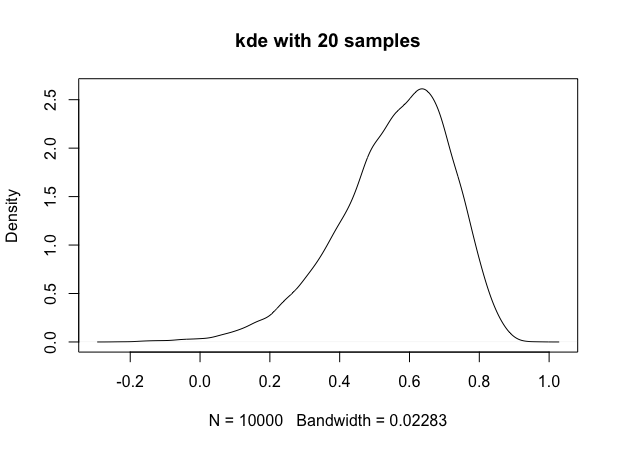
\includegraphics[width=500pt]{hw5_2a_20.png}
\end{figure}
\begin{figure}[h!]
  \centering
  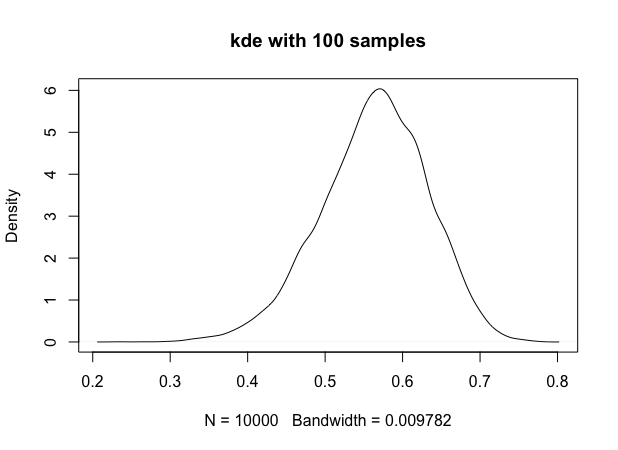
\includegraphics[width=500pt]{hw5_2a_100.png}
\end{figure}
\begin{figure}[h!]
  \centering
  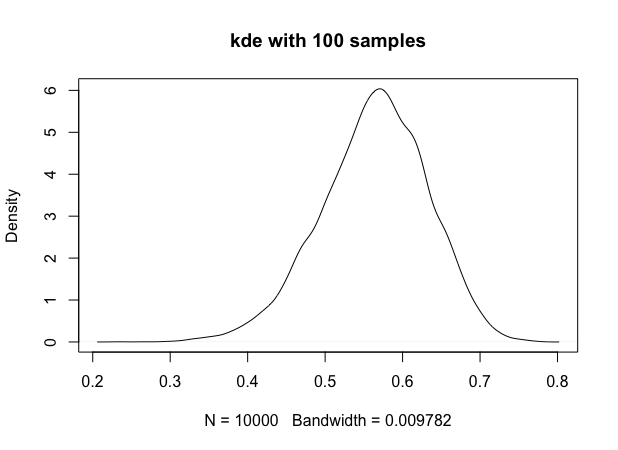
\includegraphics[width=500pt]{hw5_2a_100.png}
\end{figure}
% No clue, look at diagrams more seriously -- narrowing/expanding?
The symmetry of the distribution tends to stay the same time as $n$ increases, while the spread seems to decrease from $n = 20$ to $n = 100$, and then increase yet again from $n = 100$ to $n = 200$.

\subsection*{(b)}

We can find the variance for each $n$ to estimate $\text{se}(\hat{\rho}_n)$: \\
$\text{se}(\hat{\rho}_20) = 0.1890982$ \\
$\text{se}(\hat{\rho}_100) = 0.109021$ \\
$\text{se}(\hat{\rho}_500) = 0.08856526$ \\ \\
We can find the 

\subsection*{(c)}


}

\section*{3.}
{\Large

\subsection*{(a)}



\subsection*{(b)}



\subsection*{(c)}


}

\end{document}